%%%%%%%%%%%%%%%%%%%%%%%%%%%%%%%%%%%%%%%%%

%----------------------------------------------------------------------------------------
%	PACKAGES AND OTHER DOCUMENT CONFIGURATIONS
%----------------------------------------------------------------------------------------

\documentclass{article}

\input{C:/Code/TexStudio/templates/structure.tex} 
%% Include the file specifying the document structure and custom commands

%----------------------------------------------------------------------------------------
%	ASSIGNMENT INFORMATION
%----------------------------------------------------------------------------------------

\title{Assignment \#3} 
% Title of the assignment

\author{Name:Cao Mingming \indent \indent ID:2018311770\\ 
\texttt{cmm18@mails.tsinghua.edu.cn}} 
% Author name and email address

\date{Tsinghua University --- \today} 
% University, school and/or department name(s) and a date

%----------------------------------------------------------------------------------------

\begin{document}

\maketitle 
% Print the title
% \section*{Introduction} untitled section

\section{Problem 1}
After solving the stability condition, the Eq. (2.3) of the textbook show two solutions. However,the both of solutions cannot give a proper q-parameter, since there should be only on the size and the Radius curvature of the beam shown in the Eq. (2.4) and Eq. (2.5). Then what would be the proper way of understanding the two solutions in the Equation. (2.3)?

\section*{Sloution}
From the previous chapter q can be written in the form of,
\begin{equation}\label{eq1}
	q_1=\frac{1}{q}=\frac{1}{R}-i\frac{\lambda}{n\pi\omega^2}.
\end{equation}
The solution of stable condition indicates that,
\begin{equation}\label{eq2}
	\begin{array}{l}
		q_1=\frac{D-A}{2B}\pm\frac{1}{2B}\sqrt{\Delta^2}
		\\
		\\
		\Delta^2=(A-D)^2+4BC
	\end{array}
\end{equation}
If $\Delta^2\l 0$, $q_1$ is a real number which cannot be q parameter. So we could get that $\Delta^2\l0$. And due to the determinant of ABCD matrix is 1, we can rewrite $\Delta^2=(A+D)^2-4$.
Now we can rewrite the solution as,
\begin{equation}\label{eq3}
	q_1=q_1=\frac{D-A}{2B}\pm i\frac{1}{2B}\sqrt{4-(A+D)^2}.
\end{equation}
Compare equation \ref{eq3} with equation \ref{eq1} we can get that,
\begin{equation}
	\begin{array}{l}
		R=\frac{2B}{D-A}
		\\
		\\
		\omega=\sqrt{\frac{2\lambda|B|}{4-(A+D)^2}}
	\end{array}
\end{equation}
The pluse one of the equation \ref{eq2} can ignore for that its propagation direction is oppsite to real propagation direction.

\section{Problem 2}
Is the complex q parameter in the cavity dependent on the direction of the laser beam?
\begin{figure}
	\centering
	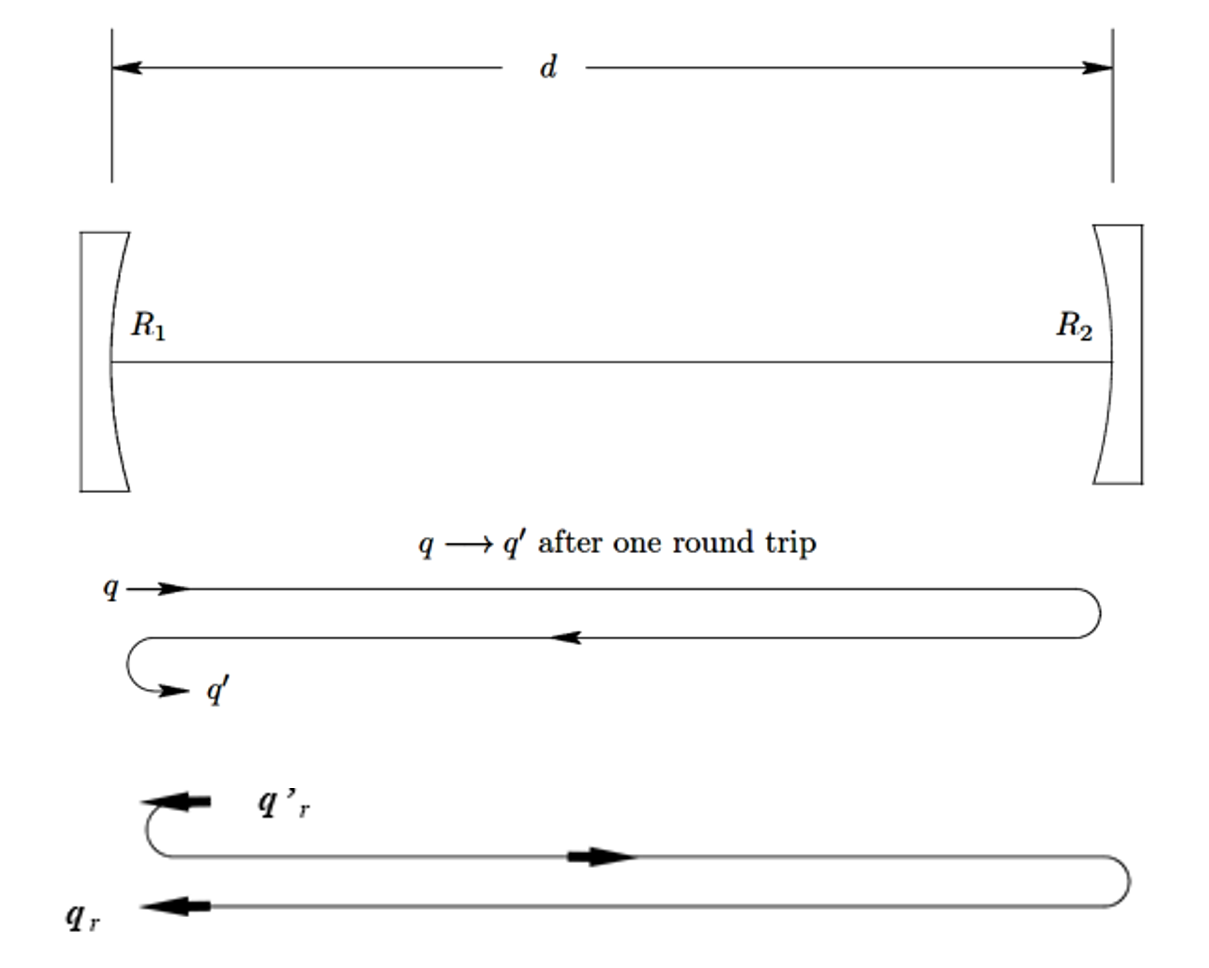
\includegraphics[width=10cm]{q22.png}
	\caption{Question 2}
\end{figure}
As an example, in the above figure, the q parameter in the case of (a) would be same or different from the $q_r$ parameter in the case of (b)? Find both q and q r parameters from the self-consistent solution and conclude that they are same or different.
\section*{Solution}
For the case (a), ABCD matrix can be written as,
\begin{equation}
	M_1=
	\begin{pmatrix}
		1              & 0\\
		-\frac{2}{R_1} & 1
	\end{pmatrix}
	\begin{pmatrix}
		1 & d\\
		0 & 1
	\end{pmatrix}
	\begin{pmatrix}
		1 & 0\\
		-\frac{2}{R_2} & 1
	\end{pmatrix}
	\begin{pmatrix}
		1 & d\\
		0 & 1
	\end{pmatrix}
\end{equation}
Let,
\begin{equation}
	g1=1-\frac{d}{R_1}\quad g_2=1-\frac{d}{R_2}
\end{equation}
we can get,
\begin{equation}\label{eq4}
	M_1=
	\begin{pmatrix}
		A & B\\
		C & D
	\end{pmatrix}
	=
	\begin{pmatrix}
		2g_2-1 & 2g_2d \\
		\frac{2}{d}(2g_{1}g_{2}-g_{1}-g_{2}) & 4g_{1}g_{2}-2g_2-1
	\end{pmatrix}
\end{equation}
Take equation \ref{eq4} into equation \ref{eq2},
\begin{equation}\label{eq5}
	q_1=\frac{g_1-1}{d}\pm i\frac{1}{g_2d}\sqrt{g_{1}g_{2}(1-g_1g_{2})}.
\end{equation}
If we change the direction of laser beam, the ABCD matrix along the propagation direction is,
\begin{equation}\label{key}
	M_2=
	\begin{pmatrix}
	A & B\\
	C & D
	\end{pmatrix}
	=
	\begin{pmatrix}
	1 & d\\
	0 & 1
	\end{pmatrix}
	\begin{pmatrix}
	1 & 0\\
	-\frac{2}{R_2} & 1
	\end{pmatrix}
	\begin{pmatrix}
	1 & d\\
	0 & 1
	\end{pmatrix}
		\begin{pmatrix}
	1              & 0\\
	-\frac{2}{R_1} & 1
	\end{pmatrix}
\end{equation}
simplifying above equation we could get,
\begin{equation}
	M_2=
	\begin{pmatrix}
	A & B\\
	C & D
	\end{pmatrix}
	=
	\begin{pmatrix}
	4g_{1}g_{2}-2g_2-12g_2-1 & 2g_2d \\
	\frac{2}{d}(2g_{1}g_{2}-g_{1}-g_{2}) & 2g_2-1
	\end{pmatrix}
\end{equation}
Compare with $M_1$ we find that A exchanges position with D in $M_2$, and using  equaiton 3 we could get,
\begin{equation}
	q_{r1}=-\frac{g_1-1}{d}\pm i\frac{1}{g_2d}\sqrt{g_{1}g_{2}(1-g_1g_{2})}.
\end{equation}
So we can find that $q_1$ and $q_{r1}$ has the same beam size but their radius of curvature are the oppsite number which is caused by the opposite propagtion direction.
\section{Probelm 3}
In the following optical resonator, find the radius of curvature $R(z)$ and width $ w(z) $ in terms of $ z  $ and draw graphs such as $ R(z) $ vs $  z $ and $ w(z) $  vs  $ z $. You may choose the values of $ R_1 ,R_2 $ , and d in the stable condition (e.g. $ R_1 = 10 cm, R_2 = 12 cm, d = 8 cm, \lambda= 1 \mu m $).
\begin{figure}[htb]
	\centering
	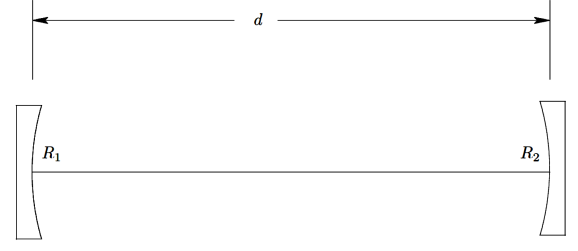
\includegraphics[width=8cm]{question3.png}
	\caption{Question 3}
\end{figure}

\section*{Solution}
Assume that the laser beam starts from the left hand of the cavity, the distance there is $z_1$, according to chapter 1,
\begin{equation}
	q(z)=q_0+z=i z_R+z
\end{equation}
From equation \ref{eq5} we can get that,
\begin{equation}
	q_1=\frac{1}{q(z_1)}=\frac{g_1-1}{d}- i\frac{1}{g_2d}\sqrt{g_{1}g_{2}(1-g_1g_{2})}.
\end{equation}
So we can get,
\begin{equation}\label{eq6}
	\begin{array}{l}
		z_1=-\frac{Re(q_1)}{|q_1|^2}=d\frac{g_2(g_1-1)}{g_1+g_2-2g_1g_2}\\
		\\
		z_R=d\frac{\sqrt{g_1g_2(1-g_1g_2)}}{g_1+g_2-2g_1g_2}
	\end{array}
\end{equation}
And,
\begin{equation}\label{eq7}
	\begin{aligned}
		q(z)&=i z_R+z \\
		\\
		&=i d\frac{\sqrt{g_1g_2(1-g_1g_2)}}{g_1+g_2-2g_1g_2}+z
	\end{aligned}
\end{equation}
compare eqaution \ref{eq7} with
$$
q_1=\frac{1}{q}=\frac{1}{R}-i\frac{\lambda}{n\pi\omega^2}
$$
we can get,
\begin{equation}\label{eq8}
	\begin{array}{l}
		R(z)=z+\frac{z_R^2}{z}\\
		\\
		\omega(z)=\sqrt{\frac{\lambda}{n\pi}(z_R+\frac{z^2}{z_R})}
	\end{array}
\end{equation}
By eqaution \ref{eq7} we can draw the picture as following.
\begin{figure}[h]
	\centering
	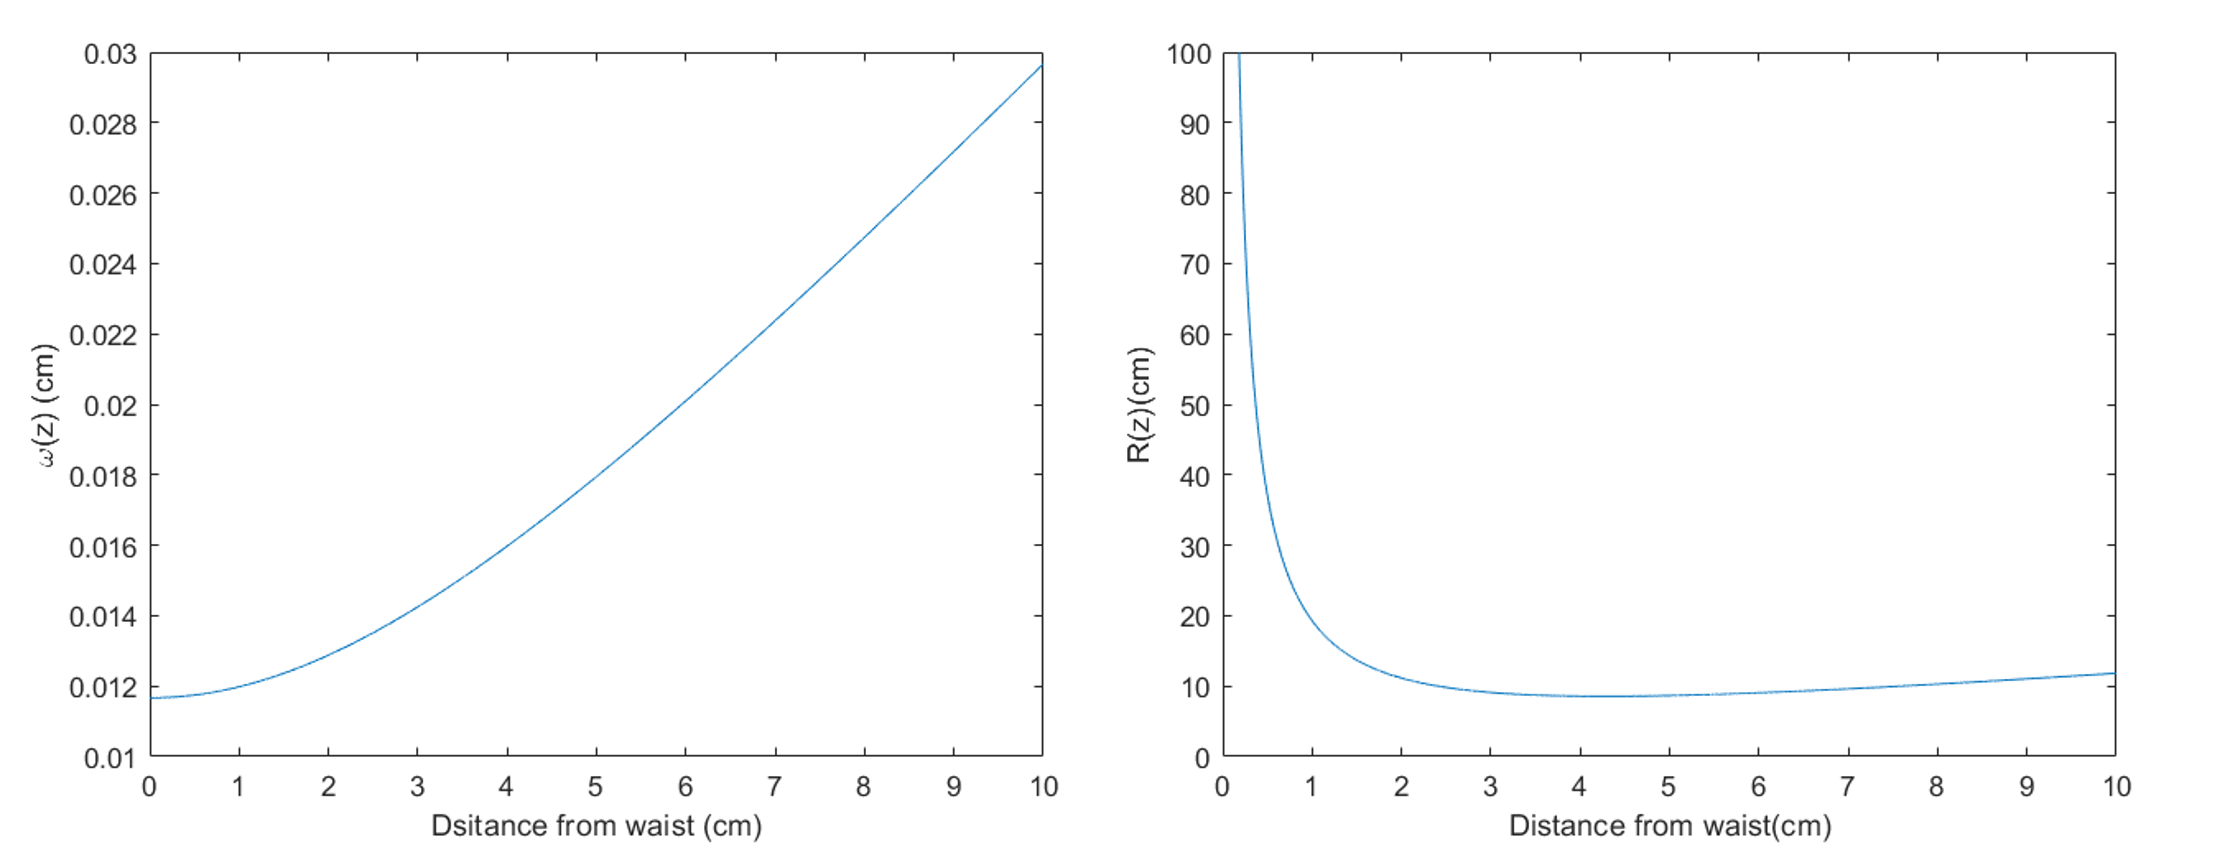
\includegraphics[width=14cm]{figure.png}
	\caption{Figure of $R(z)$ and $\omega(z)$}
\end{figure}

\section{Problem 4}
In the above optical resonator, discuss the location of the beam waist in the case of $R_1 \leq R_2$ . The location is clear to mirror $ R_1 $ or $ R_2 $ ?
\section*{Solution}
We have set location of beam waist as the zero point of $z$ In the above optical cavity. And we have calculated the distance of mirror $R_1$ from the beam waist as equation  \ref{eq6}. The length of the cavity is $d$,so we could get the distance of mirror $R_2$ from the waist as $z_1+d$,
\begin{equation}\label{eq8}
	\begin{aligned}
	z_2&=z_1+d\\
	\\
	&=d\frac{g_1(1-g_2)}{g_1+g_2-2g_1g_2}
	\end{aligned}
\end{equation}
To compare which one is closer to the beam waist, let
\begin{equation}\label{key}
	\begin{aligned}
	k&=\frac{|z_1|}{|z_2|}\\
	\\
	&=\frac{|1-\frac{1}{g_1}|}{|1-\frac{1}{g_2}|}\\
	\\
	&=\frac{|R_2-d|}{|R_1-d|}
	\end{aligned}	
\end{equation}
So we could get the conclusion that,
\begin{itemize}
	\item case 1: $d<R_1<R_2$\quad k>1,\quad $z_2$ is closer.
	\item case 2: $R_1<R_2<d$\quad k<1,\quad $z_1$ is closer.
\end{itemize}
 %----------------------------------------------------------------------------------------
%	PROBLEM 1
%----------------------------------------------------------------------------------------

\end{document}

